\chapter{API, OPERACIONES CRUD Y DASHBOARD}
\label{cap:aplicacion}
\section{Capa de consulta y acceso}
El dashboard usa React, TypeScript, componentes shadcn/ui, Recharts y un grafo interactivo. nginx sirve la aplicación y redirige \codigo{/api} a FastAPI. El navegador no abre conexiones directas con las bases: la API centraliza consultas, conversiones temporales y operaciones de escritura \cite{repo}.

El módulo \ruta{api/queries.py} conserva conexiones y utiliza una caché breve para consultas repetidas. Las mutaciones CRUD limpian esa caché. Los filtros se validan en el servidor; los valores entran como parámetros a las consultas y los tipos de relación y columnas editables se restringen mediante listas permitidas.

Cuando \codigo{DASHBOARD_PASSWORD} está definida, la API requiere una cookie de sesión para las rutas protegidas. La clave es compartida por el equipo; el código no implementa cuentas individuales ni permisos por rol. La cookie usa \codigo{HttpOnly} y \codigo{SameSite=Lax}. Los archivos de despliegue revisados no incluyen terminación TLS, por lo que un uso fuera de la demostración requiere completar esa protección y la administración de identidades.

\section{Operaciones CRUD en MongoDB}
La interfaz ofrece formulario y JSON sincronizados para crear eventos de los cuatro tipos. El servidor calcula \codigo{derived}; el usuario no necesita escribirlo manualmente. Un documento incompleto permite demostrar el rechazo del validador. Los duplicados de \codigo{_id} se informan como conflicto.

La consulta admite wiki, tipo, editor, título, período, demostración e identificador. El detalle expone el documento. En una actualización se aceptan rutas como \codigo{length.new}; se protegen \codigo{_id}, \codigo{meta.id} y \codigo{derived}. El servidor simula el nuevo documento, recalcula los derivados necesarios y retira los campos derivados que ya no correspondan.

La eliminación muestra el registro y requiere confirmación en la interfaz. Modificar un evento cambia MongoDB de inmediato, pero no reconstruye automáticamente Cassandra y Neo4j; el usuario operador debe reprocesar las horas afectadas para actualizar resultados consolidados.

\begin{figure}[H]
\centering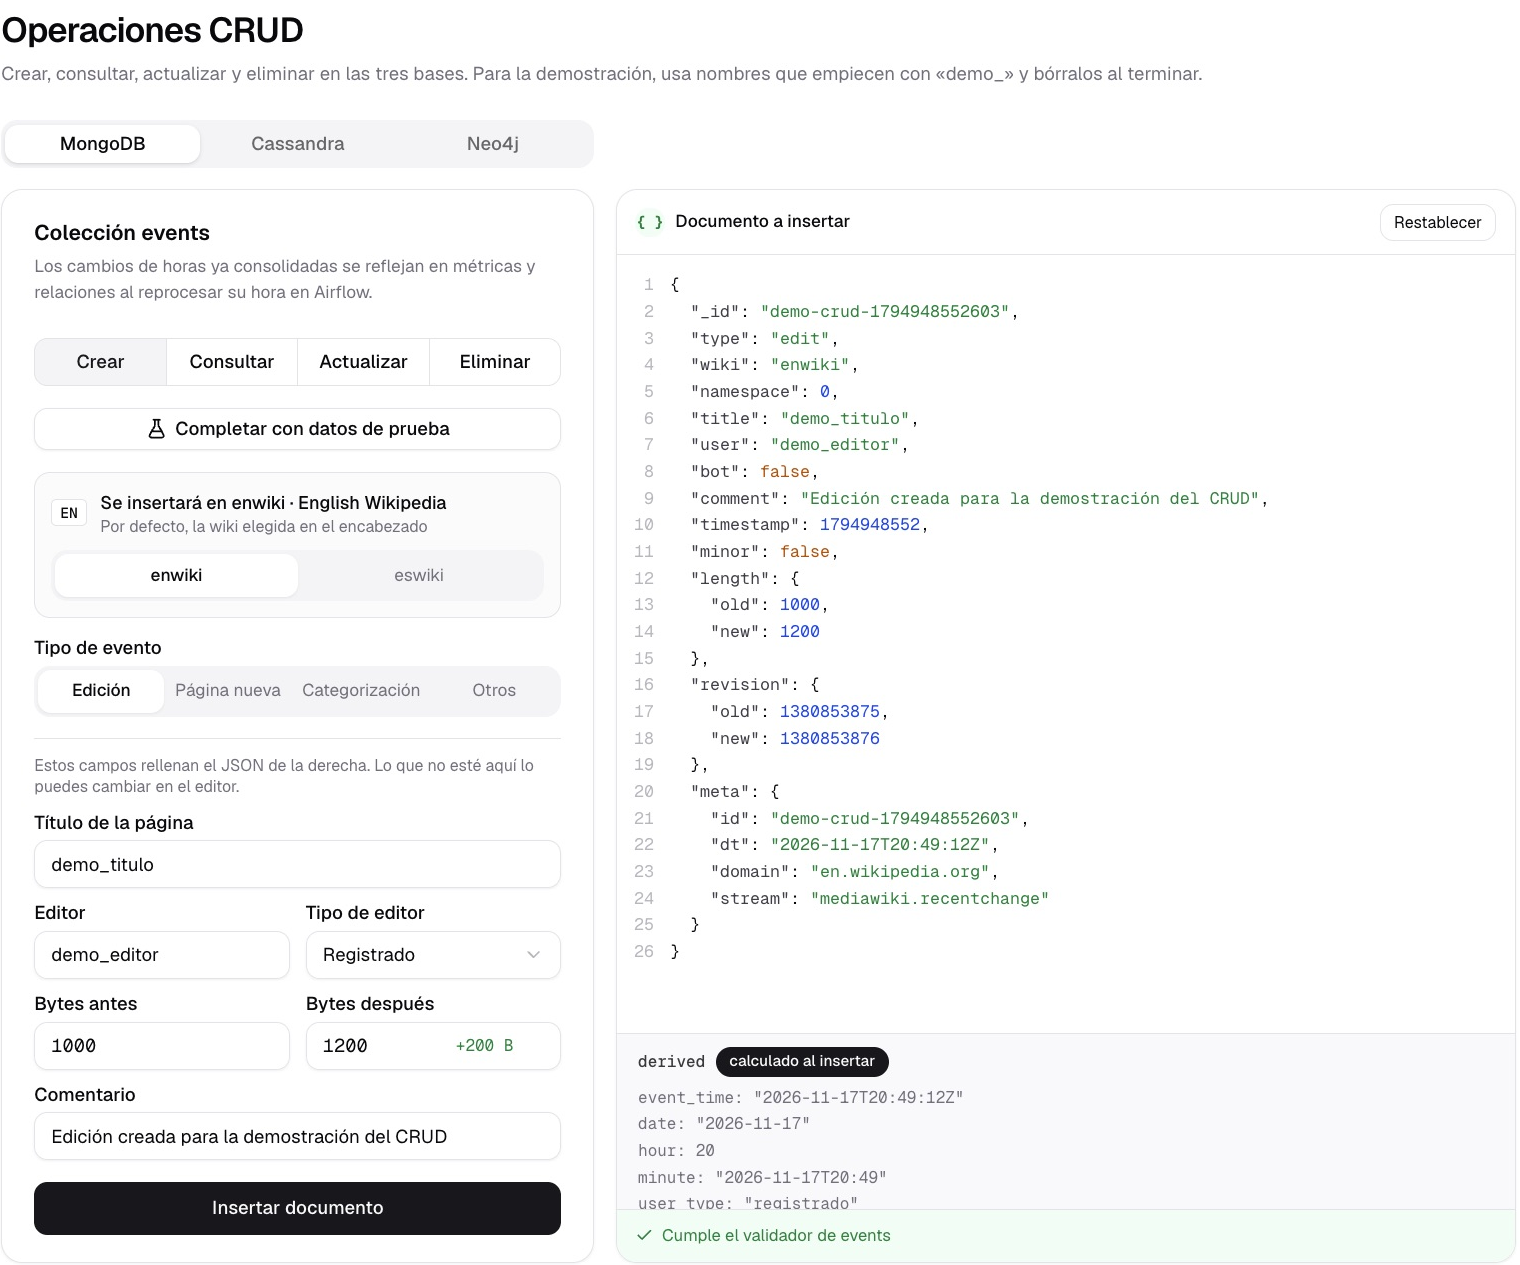
\includegraphics[width=0.94\textwidth,height=0.62\textheight,keepaspectratio]{dashboard-crud-mongo.png}
\caption{MongoDB: formulario y documento JSON de una creación.}\label{fig:ui-mongo}
\fuente{dashboard del proyecto desplegado en Google Cloud Platform}
\end{figure}

\section{Operaciones CRUD en Cassandra}
El CRUD vigente trabaja sobre \codigo{kpis}, cuya clave completa es \codigo{(kpi,ventana)}. La inserción permite crear una fila y también reemplazar una clave existente. La consulta accede a una partición y opcionalmente a un día y una hora UTC. La API normaliza la ventana al inicio horario.

La actualización admite únicamente \codigo{valor} y \codigo{detalle}, verifica que la fila exista y rechaza valores incompatibles. Esta comprobación evita que un \codigo{UPDATE} sobre una clave ausente se interprete en la interfaz como modificación de un registro previo. Se puede eliminar una fila con la clave completa o toda la partición si solo se indica el KPI.

Se recomienda utilizar nombres \codigo{demo_} en la exposición. El código actual reconoce ese prefijo para organizar registros de demostración, pero no impone una prohibición general de escribir otros nombres. Algunas notas históricas describen una restricción anterior que ya no corresponde al comportamiento actual.

\begin{figure}[H]
\centering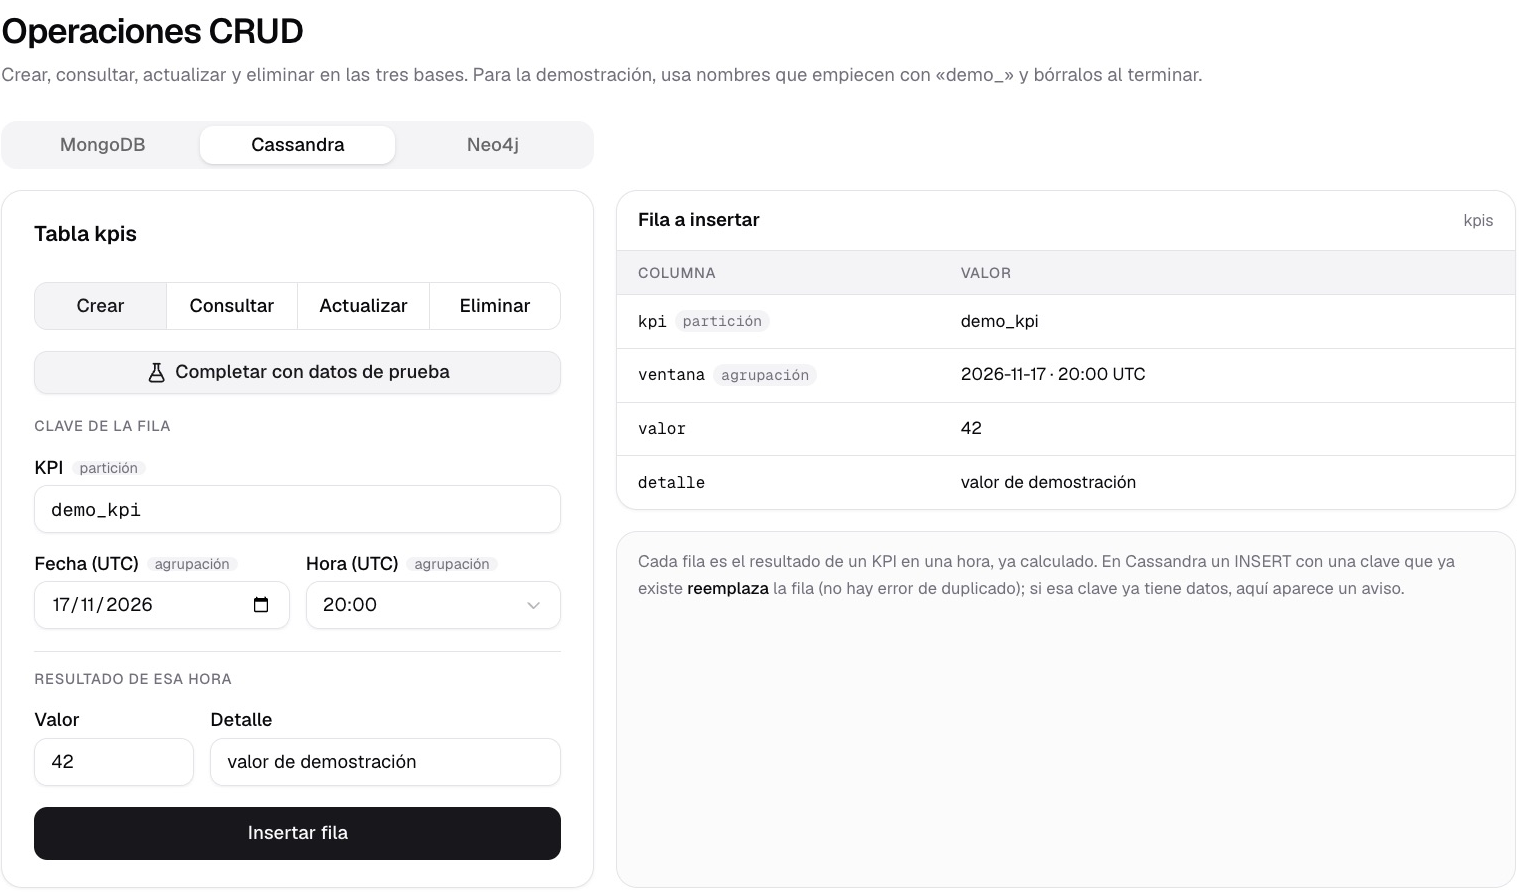
\includegraphics[width=0.96\textwidth,height=0.57\textheight,keepaspectratio]{dashboard-crud-cassandra.png}
\caption{Cassandra: clave, valor y vista previa de una fila de KPI.}\label{fig:ui-cassandra}
\fuente{dashboard del proyecto desplegado en Google Cloud Platform}
\end{figure}

\section{Operaciones CRUD en Neo4j}
La interfaz crea nodos \codigo{Editor}, consulta sus vecinos, actualiza propiedades y permite crear o eliminar relaciones entre editores. Las relaciones de interfaz incluyen \codigo{REVIRTIO}, \codigo{MENSAJE_A}, \codigo{AGRADECIO} y \codigo{BLOQUEO}; la biblioteca de consola también permite relacionar un editor con una página mediante \codigo{EDITO}.

La creación de una relación puede asegurar que existan sus extremos y marca la relación como manual. La consulta muestra un grafo y sus propiedades. El nombre \codigo{user} se protege como identidad del nodo al actualizarlo. Para eliminar un nodo se usa \codigo{DETACH DELETE}, que retira también sus relaciones.

El modelo temporal puede contener varias relaciones del mismo tipo entre dos nodos. Por ello, la eliminación acepta \codigo{elementId} y exige seleccionar una relación cuando hay ambigüedad. Esta distinción evita borrar simultáneamente contribuciones de horas o wikis diferentes.

\begin{figure}[H]
\centering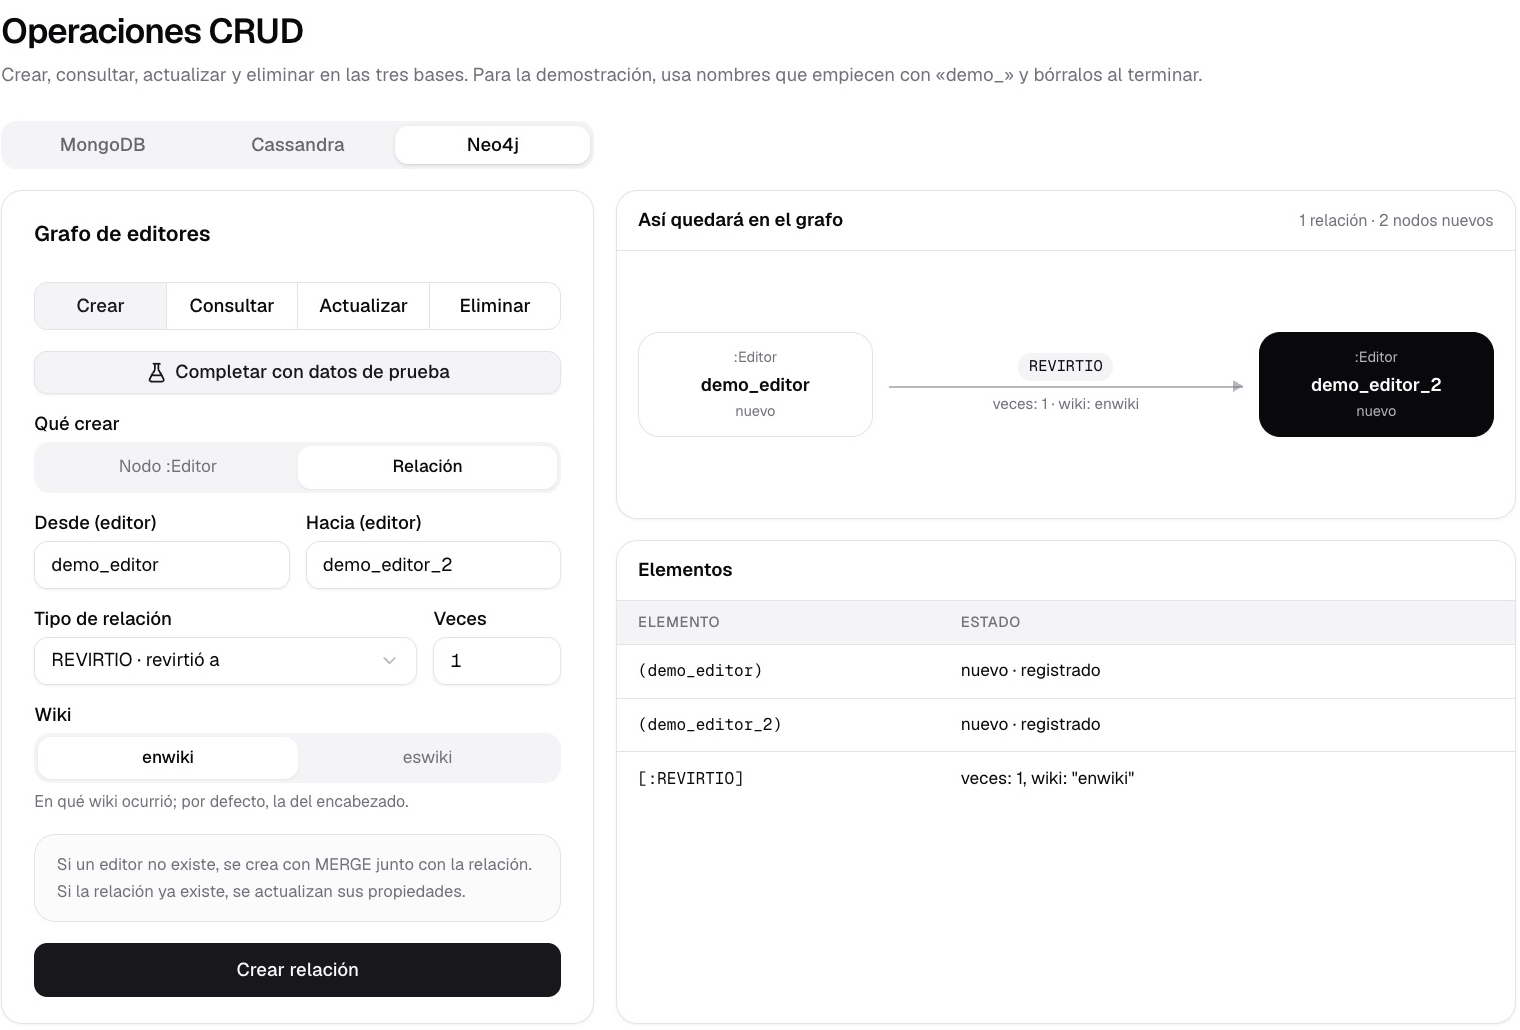
\includegraphics[width=0.96\textwidth,height=0.60\textheight,keepaspectratio]{dashboard-crud-neo4j.png}
\caption{Neo4j: creación de relaciones y vista previa del grafo.}\label{fig:ui-neo4j}
\fuente{dashboard del proyecto desplegado en Google Cloud Platform}
\end{figure}

\begin{tabla}
\begin{tabularx}{\textwidth}{P{2.2cm}YYY}
\toprule
Operación & MongoDB & Cassandra & Neo4j \\
\midrule
Crear & Insertar documento. & Insertar o reemplazar fila. & Crear nodo o relación. \\
Consultar & Leer documento o búsqueda filtrada. & Leer partición o clave completa. & Leer nodo, vecinos y propiedades. \\
Actualizar & Cambiar campos y recalcular derivados. & Cambiar valor o detalle. & Cambiar propiedades. \\
Eliminar & Borrar documento por identificador. & Borrar fila o partición. & Borrar una relación o nodo con sus relaciones. \\
\bottomrule
\end{tabularx}
\caption{Correspondencia funcional de las operaciones CRUD.}
\end{tabla}

La demostración por consola se ejecuta con \codigo{python -m wikipipe.crud todo}. Crea entidades de prueba, consulta el resultado, las modifica y las retira. No se ejecutó sobre una instalación productiva durante la elaboración de este informe.

\section{Vistas analíticas y operativas}
\subsection{Resumen y KPIs}
Presenta dos períodos: última hora consolidada y acumulado hasta un cierre identificado. Las cuatro tarjetas principales se complementan con detalles, protagonistas, evolución por hora y ejecuciones. Los protagonistas de la hora usan exclusivamente esa ventana. En el acumulado, los porcentajes se obtienen a partir de totales, evitando promediar porcentajes horarios.

Hay una diferencia entre el KPI histórico \codigo{total_eventos_acumulados}, que cuenta documentos de MongoDB anteriores al cierre, y las tarjetas acumuladas de la versión actual, que suman únicamente horas completadas del modelo 2. Sus cifras pueden diferir si existen eventos almacenados en ventanas todavía no consolidadas.

\subsection{En vivo}
Muestra eventos y participación de los últimos cinco minutos frente a los cinco anteriores. Ambos intervalos comparten un único instante de corte y no se superponen. Las tarjetas de editores cuentan participantes distintos en cada intervalo, no usuarios conectados a Wikipedia. La serie de treinta minutos aporta contexto y los filtros permiten revisar tipos, cuentas y borrados grandes.

La vista combina documentos y conteos provisionales. No debe compararse como si representara una hora completa ni interpretarse como una medición de latencia garantizada.

\subsection{Actividad en el tiempo}
Presenta el día local con horas consolidadas, evolución por minuto y páginas activas. Los eventos pendientes se informan aparte. El promedio por minuto divide entre el número de horas consolidadas multiplicado por 60, incluidos los minutos sin eventos. La comparación diaria utiliza las mismas horas del día anterior cuando la cobertura permite hacerlo.

\subsection{Explorador de eventos}
Consulta MongoDB y muestra composición por tipo sobre todo el dataset de las wikis elegidas. El total y los tipos salen de una misma agregación. Los filtros de búsqueda restringen la tabla de resultados, sin cambiar ese resumen general. La ficha permite revisar JSON y campos derivados.

\subsection{Red de editores}
Combina tarjetas de las últimas 24 horas hasta el cierre disponible con rankings de todo el historial conservado y la red alrededor de una cuenta. Los textos identifican esos alcances distintos. Se visualizan reversiones, mensajes, agradecimientos, bloqueos y coedición. La vista actual no presenta el ranking de páginas disputadas, aunque una consulta relacionada permanece disponible en la API.

\subsection{Operaciones CRUD y Arquitectura}
CRUD reúne formularios, previsualización y resultados de las tres bases. Arquitectura muestra componentes, conexiones y explicaciones de la fuente, almacenamiento, API y proceso horario. Sus pestañas permiten alternar el diagrama del despliegue y el funcionamiento lógico. Estas vistas facilitan la demostración técnica y la inspección del sistema.

\begin{tabla}
\begin{tabularx}{\textwidth}{P{3.5cm}P{3.7cm}Y}
\toprule
Vista & Fuente predominante & Período principal \\
\midrule
Resumen y KPIs & Cassandra, control en MongoDB y protagonistas de grafo/documentos. & Hora consolidada o acumulado al corte. \\
En vivo & MongoDB y minutos de Cassandra. & Cinco minutos; serie de treinta minutos. \\
Actividad & Cassandra y ventanas completadas. & Día local con horas consolidadas. \\
Explorador & MongoDB. & Dataset almacenado y búsqueda. \\
Red de editores & Neo4j y resúmenes de Cassandra. & Tarjetas de 24 h; rankings históricos. \\
CRUD & Las tres bases. & Registro o entidad seleccionada. \\
Arquitectura & Código y metadatos de las bases. & Estado y diseño del sistema. \\
\bottomrule
\end{tabularx}
\caption{Fuentes y alcance temporal de las siete vistas.}
\end{tabla}

\Needspace{18cm}
\section{Capturas y lectura de la interfaz}
Las figuras de este capítulo se obtuvieron del dashboard del proyecto desplegado en Google Cloud Platform, disponible en la dirección de la aplicación~\cite{dashboard}. Muestran los formularios CRUD y el recorrido de los datos entre los componentes del sistema.

\begin{figure}[H]
\centering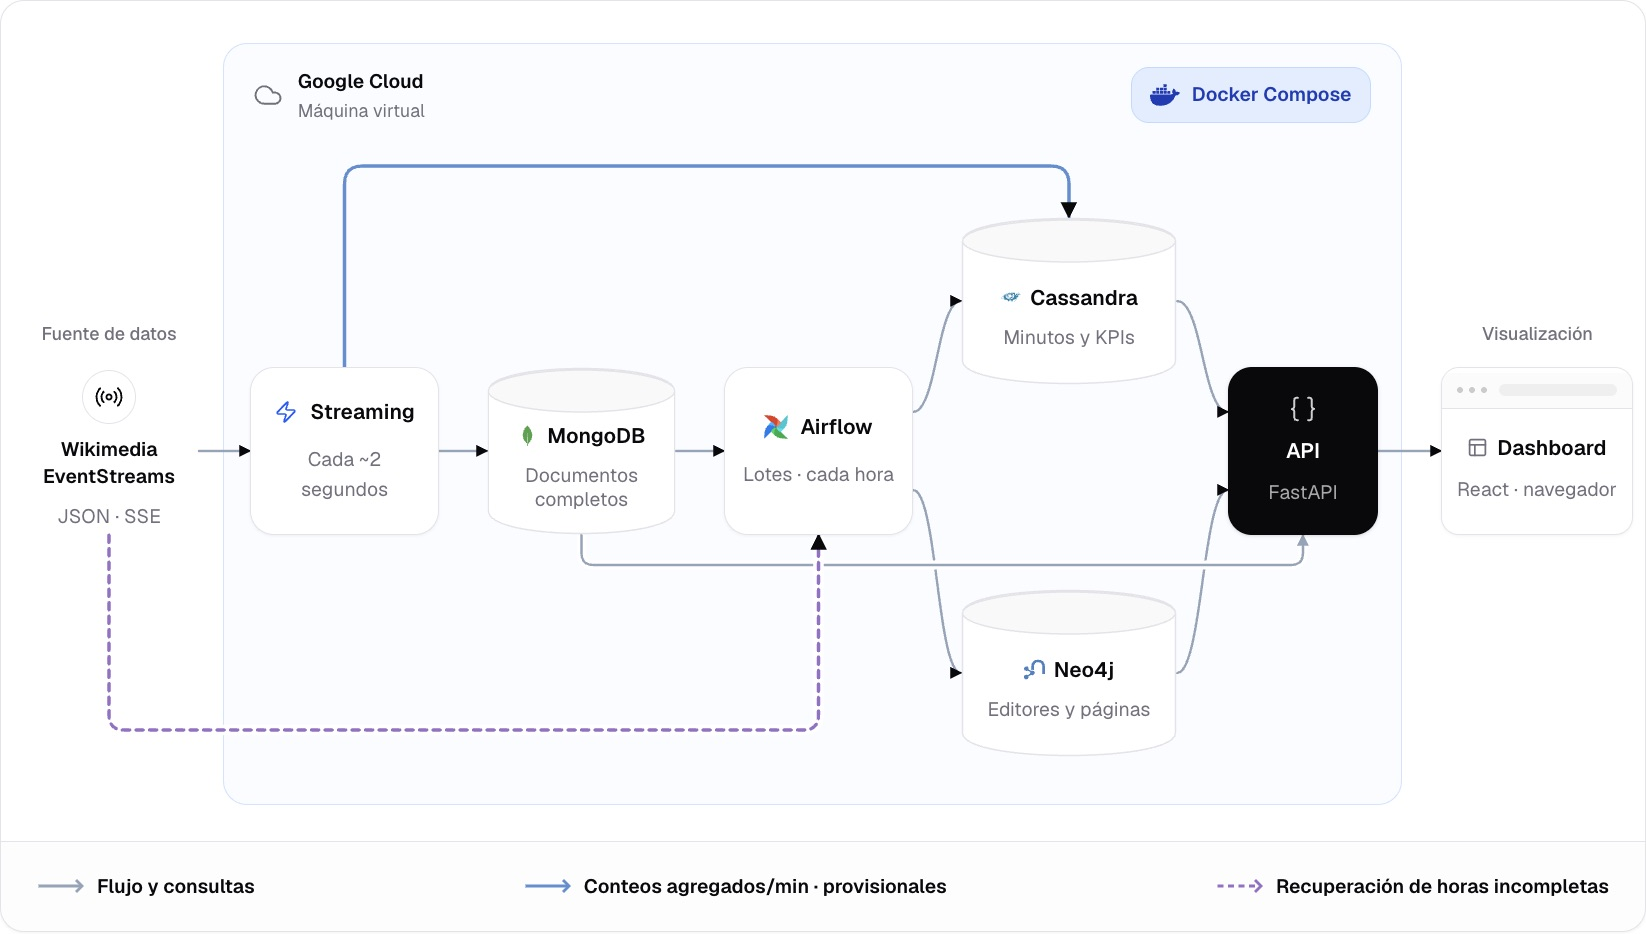
\includegraphics[width=\textwidth]{dashboard-arquitectura.png}
\caption{Arquitectura: recorrido de los datos y componentes del sistema.}\label{fig:ui-arq}
\fuente{dashboard del proyecto desplegado en Google Cloud Platform}
\end{figure}

La vista distingue tres recorridos: ingesta continua, consolidación horaria y consulta. Las flechas identifican los conteos provisionales y la recuperación de ventanas incompletas. Los componentes abren explicaciones de su función, mientras las pestañas permiten alternar la infraestructura y el proceso lógico.
